\documentclass{beamer}

\usepackage{graphicx}
\usepackage{textpos}
\usepackage{listings}
\usepackage{lstautogobble}

\usetheme{Madrid}
\useoutertheme{miniframes} % Alternatively: miniframes, infolines, split

% Setup the university's color pallette
\definecolor{UIUCorange}{RGB}{19, 41, 75} % UBC Blue (primary)
\definecolor{UIUCblue}{RGB}{232, 74, 39} % UBC Grey (secondary)

\definecolor{codegreen}{rgb}{0,0.6,0}
\definecolor{codegray}{rgb}{0.5,0.5,0.5}
\definecolor{codepurple}{rgb}{0.58,0,0.82}
\definecolor{backcolour}{rgb}{0.95,0.95,0.92}

\lstdefinestyle{python}{
    backgroundcolor=\color{backcolour},   
    commentstyle=\color{codegreen},
    keywordstyle=\color{magenta},
    numberstyle=\tiny\color{codegray},
    stringstyle=\color{codepurple},
    basicstyle=\ttfamily\footnotesize,
    breakatwhitespace=false,         
    belowskip=-0.5em,
    breaklines=true,                 
    captionpos=b,                    
    keepspaces=true,                 
    numbers=left,                    
    numbersep=5pt,                  
    showspaces=false,                
    showstringspaces=false,
    showtabs=false,                  
    tabsize=2
}

\lstset{style=python}

\AtBeginSection[]{
    \begin{frame}
        \vfill
        \centering
        \begin{beamercolorbox}[sep=8pt,center,shadow=true,rounded=true]{title}
            \usebeamerfont{title}\insertsectionhead\par%
        \end{beamercolorbox}
        \vfill
    \end{frame}
}
% Setup the university's color pallette
\definecolor{UIUCorange}{RGB}{19, 41, 75} % UBC Blue (primary)
\definecolor{UIUCblue}{RGB}{232, 74, 39} % UBC Grey (secondary)


\setbeamercolor{palette primary}{bg=UIUCorange,fg=white}
\setbeamercolor{palette secondary}{bg=UIUCblue,fg=white}
\setbeamercolor{palette tertiary}{bg=UIUCblue,fg=white}
\setbeamercolor{palette quaternary}{bg=UIUCblue,fg=white}
\setbeamercolor{structure}{fg=UIUCorange} % itemize, enumerate, etc
\setbeamercolor{section in toc}{fg=UIUCblue} % TOC sections

\setbeamercolor{subsection in head/foot}{bg=UIUCorange,fg=UIUCblue}
\setbeamercolor{subsection in head/foot}{bg=UIUCorange,fg=UIUCblue}

\usepackage[utf8]{inputenc}
\usepackage{graphicx}

%Information to be included in the title page:
\title{\textbf{The Internet}}
\author{\textbf{David H Smith IV}}
\institute[\textbf{UIUC}]{\textbf{University of Illinois Urbana-Champaign}}
\date{\textbf{Thurs, Nov 21 2021}}

\setbeamertemplate{title page}[default][colsep=-4bp,rounded=true]
\addtobeamertemplate{title page}{\vspace{3\baselineskip}}{}
\addtobeamertemplate{title page}{
    \begin{textblock*}{\paperwidth}(-1.0em, -1.2em)
        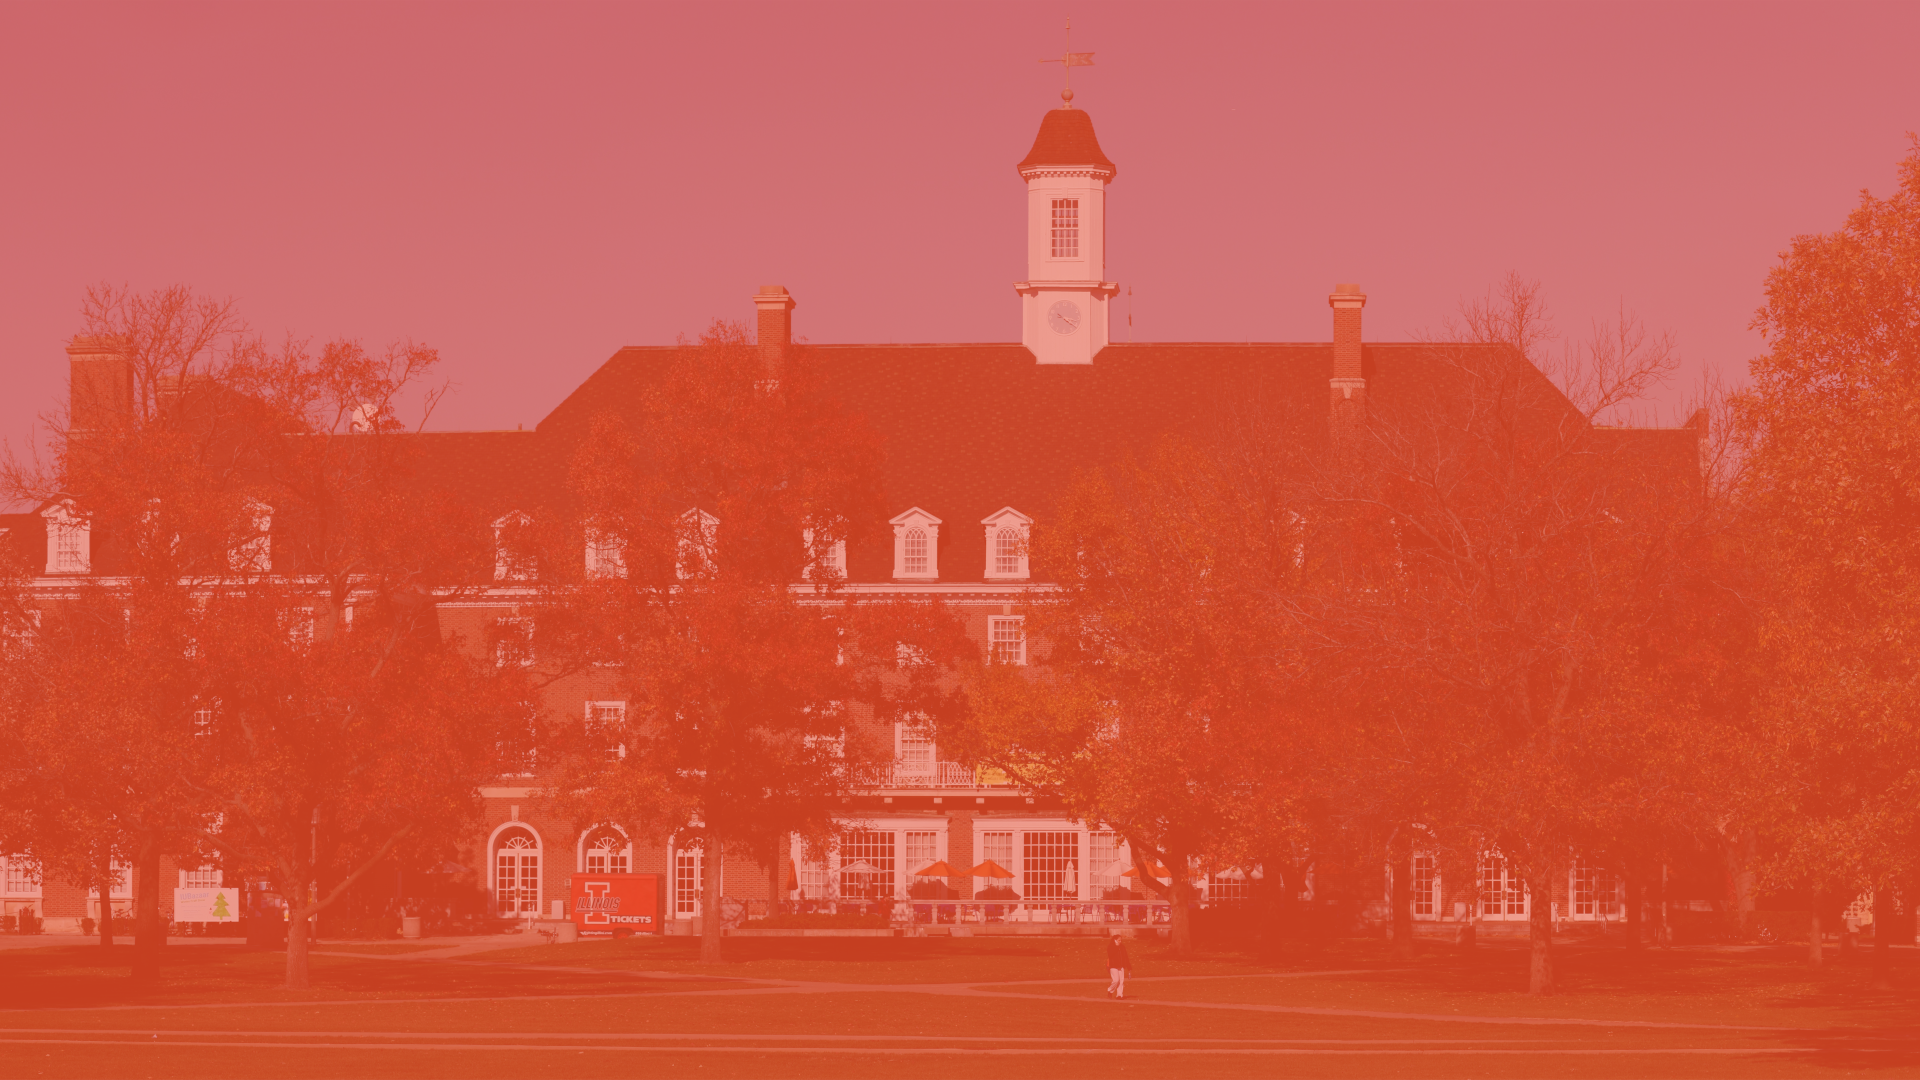
\includegraphics[width=\paperwidth, height=\paperheight]{imgs/uiuc.png}
    \end{textblock*} 
}{}

\begin{document}

\frame{\titlepage}

\section{Reminders}

%
% Slide 1
%
\begin{frame}
    \frametitle{Reminders}
    Things that are due tomorrow:
    \begin{itemize}
        \item Homework 12 
        \item Game of Life 
        \item Participation 13p1
        \item Post-reading 13p1
    \end{itemize}
\end{frame}

\section{Why we care}
%
% Slide 2
%
\begin{frame}[fragile]
    \frametitle{Where Data Comes From}
    \begin{enumerate}
        \item Started with the data being hard-coded
        \item Then we got data from the user: \lstinline|input()|
            \pause
        \item Then we got it from files: \lstinline|open(filepath)|.
            \pause
        \item Now, we can get it from the internet. The world's biggest file collection.
            \begin{itemize}
                \item Recall, websites are just collections of files on another person's computer (server):
                    \begin{lstlisting}[autogobble]
        dev_website
        |---index.html
        |___elements
            |--- about.html
            |--- cv.html
            |___ projects.html
                    \end{lstlisting} 
            \end{itemize}
    \end{enumerate}
\end{frame}

\section{History of the Internet}


%
% Slides
%
\begin{frame}[fragile]
    \frametitle{ARPANET}
    \begin{minipage}{0.48\textwidth}
        \begin{figure}
            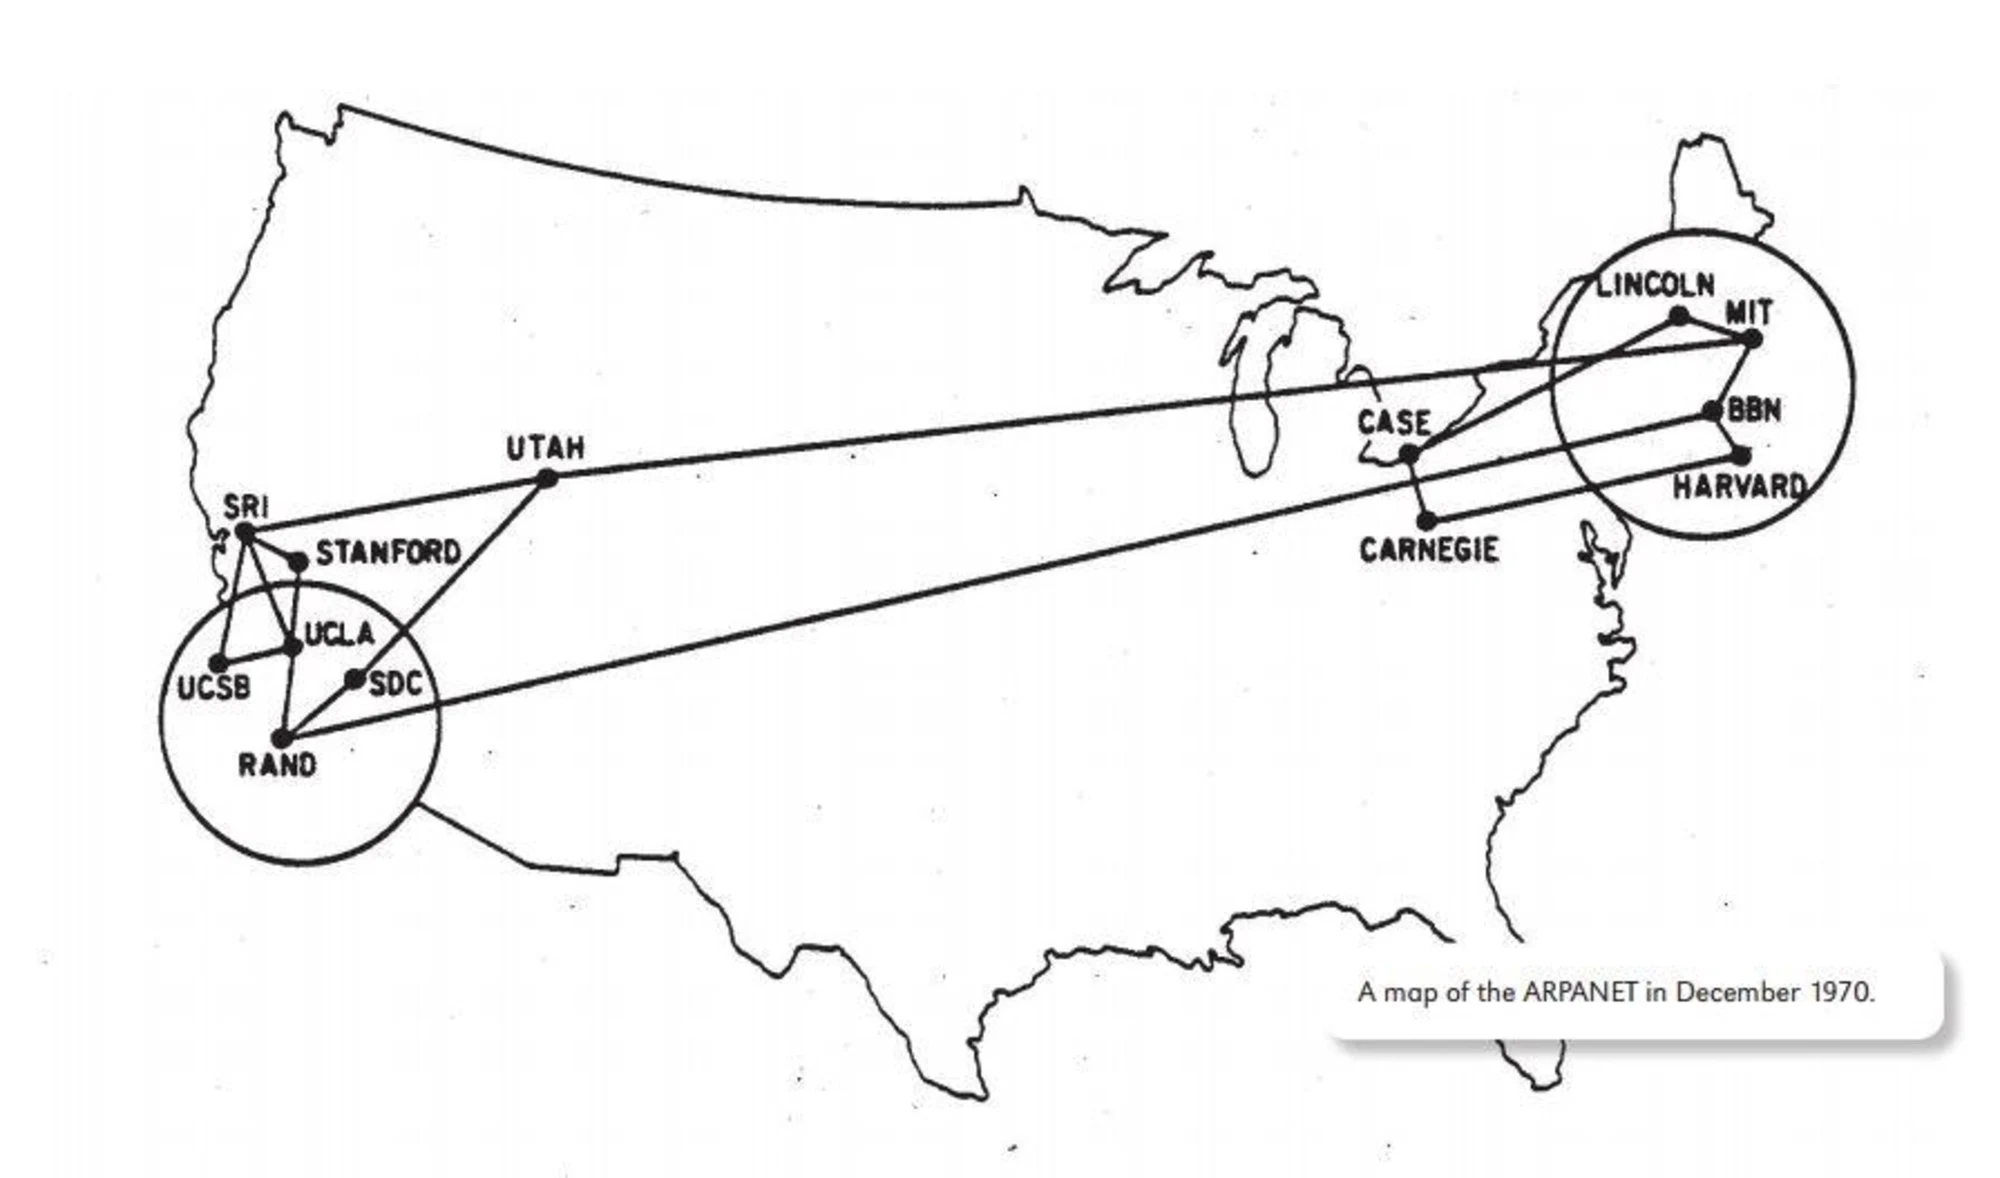
\includegraphics[width=\textwidth]{./imgs/arpanet.png}
        \end{figure}
    \end{minipage}
    \begin{minipage}{0.48\textwidth}
        \begin{itemize}
            \item Only a few users at government research facilities and universities
            \item Used for file transfer, not websites
            \item File Transfer Protocol (FTP, 1971) is still available and used today.
            \item Example: 
        \end{itemize}
    \end{minipage}
\end{frame}

%
% Slide 2
%
\begin{frame}[fragile]
    \frametitle{Tim Berners-Lee and the Internet}
    \begin{itemize}
        \item TBL was a physicist at CERN (another scientist interested in sharing work).
        \item Invented in the 1990s:
        \item Composed of the following components:
            \begin{itemize}
                \pause
                \item HTML files containing links to other HTML files
                    \pause
                    \begin{itemize}
                        \item Link: First proposed by Vannevar Bush in "As we may think".
                        \item Proposed a hypothetical machine that could let a user jump to different locations across multiple documents. Sound familiar?
                    \end{itemize}
                \item A browser, which could read and render the files.
                    \pause
                \item A set of rules (protocol), for transferring these files (HTTP).
            \end{itemize}

    \end{itemize}
\end{frame}

%
% Slide 2
%
\begin{frame}[fragile]
    \frametitle{Networks}
    \begin{minipage}{0.49\textwidth}
        \begin{figure}
            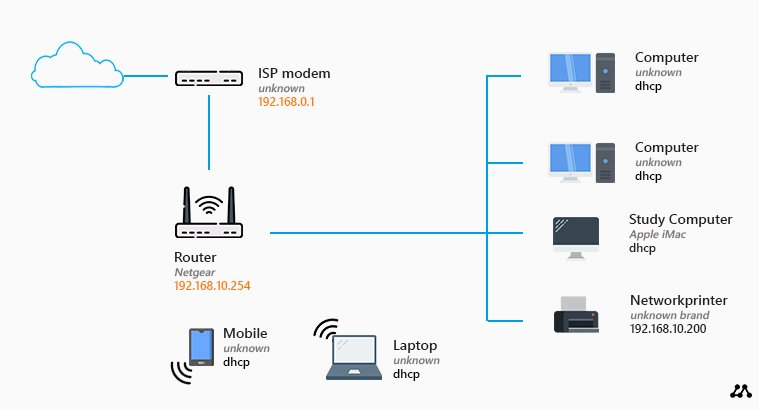
\includegraphics[width=\textwidth]{./imgs/homenetwork.jpg}
        \end{figure}
    \end{minipage}
    \begin{minipage}{0.49\textwidth}
        \begin{itemize}
                \pause
            \item Local Devices \textrightarrow \ Printers, TVs, Thermostats, Laptops, 
                \pause
            \item Router \textrightarrow \ Route data/traffic between networks.
                \pause
            \item Modem \textrightarrow \ (1) Stands for "modulation-demodulation" (2) Converts between analog (waves) and digital (10101011101).
        \end{itemize}
    \end{minipage}
\end{frame}

%
% Slide 2
%
\begin{frame}[fragile]
    \frametitle{The early internet}
    \begin{itemize}
        \item Dial-up Connections \textrightarrow  \ An internet connection that uses telephone lines as the method of connecting to the ISP. 
            \pause
        \item Bulletin Board Systems (BBS) \textrightarrow \ An early example of a server that you could run on you computer in order to allow others to use software on that server.
            \begin{itemize}
                \item These still exist and can be accessed using the "teletype network" (telnet) protocol.
                \item Telnet Example: Telnet Star Wars 
            \end{itemize}
            \pause
        \item Internet Relay Chat (IRC) \textrightarrow \ An early instant messaging system that allowed someone to use a IRC client program to connect to a server and chat.
    \end{itemize}
\end{frame}

%
% Slide 2
%
\begin{frame}[fragile]
    \frametitle{Internet Usage}
    \begin{figure}
        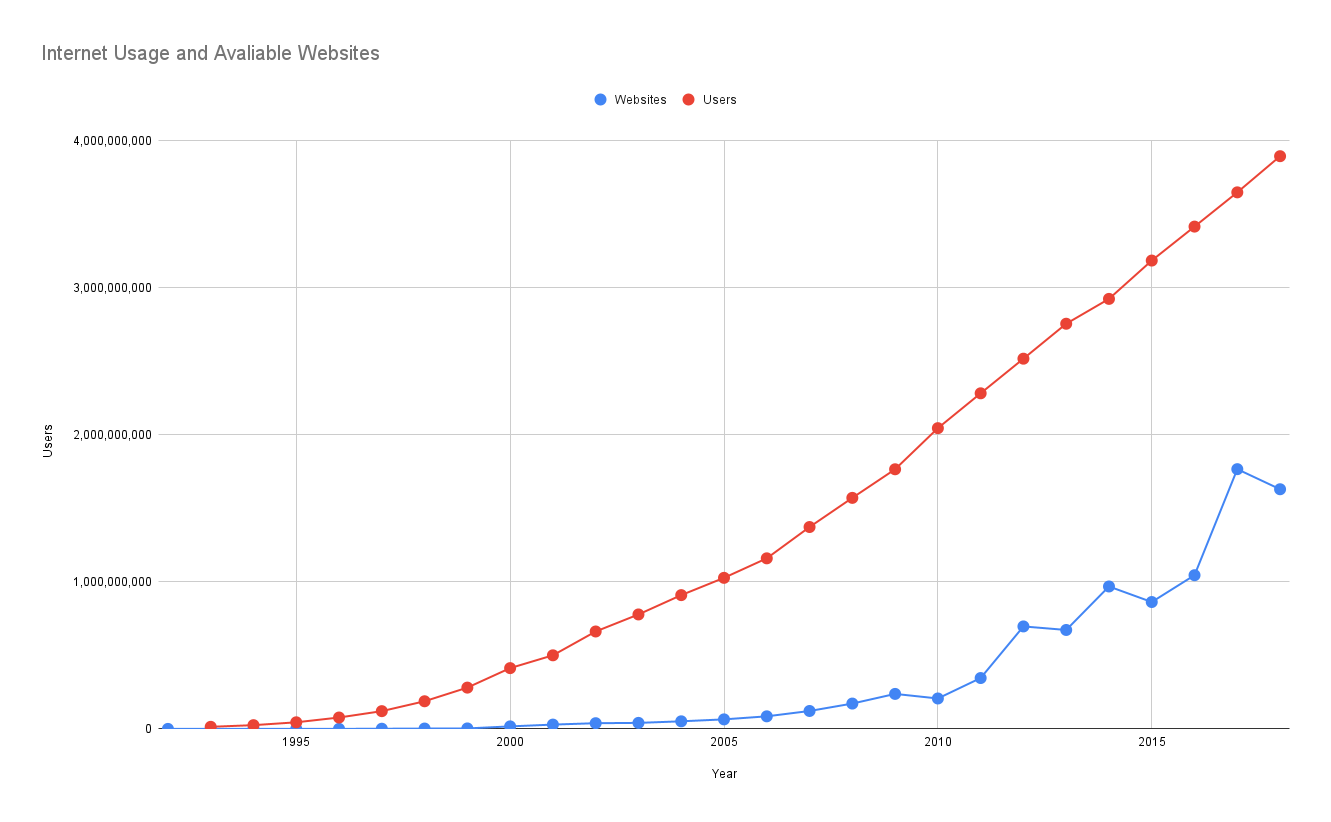
\includegraphics[width=\textwidth]{./imgs/chart.png}
    \end{figure}
\end{frame}

\section{IP Addresses, Domain Names, and URLS}

%
% Slide 2
%
\begin{frame}[fragile]
    \frametitle{IP Addresses}
    \begin{figure}
        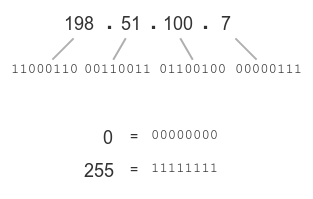
\includegraphics[width=0.35\textwidth]{./imgs/ip.png}
    \end{figure}
    \begin{itemize}
        \item Internet Protocol (IP) Address \textrightarrow \ The 32 bit (four 8-bit groups) address that specifies.
        \item Goes from 0.0.0.0-255.255.255.255
        \item Each domain name (e.g., www.google.com) has an IP address 
        \item We use a Domain Name System (DNS) server to lookup the IP attached to a domain name
    \end{itemize}
\end{frame}

%
% Slide 2
%
\begin{frame}[fragile]
    \frametitle{Domain Names}
    \begin{figure}
        \includegraphics[width=\textwidth]{./im}
    \end{figure}
    \begin{itemize}
        \item Levels of Domains:
        \begin{itemize}
            \item Top-Level Domain (TLD): .com, .edu, .net, .org 
            \item Country Code Top-Level Domain (ccTLD): .uk, .ru, .ca
            \item Second-Level Domain: google, wikipedia, youtube
            \item Sub-Domain: sub-domain(s) that fall under the second level domain. 
            \item For example, if the top and second-level domain is illinois.edu:
            \begin{itemize}
                \item cs.illinois.edu
                \item law.illinois.edu
            \end{itemize}
        \end{itemize}
    \end{itemize}
\end{frame}

%
% Slide 2
%
\begin{frame}[fragile]
    \frametitle{URLS}
    \begin{figure}
        \includegraphics[width=\textwidth]{./im}
    \end{figure}
    The Uniform Resource Locator (URL) is composed of the following parts:
    \begin{itemize}
        \item \textbf{Protocol Scheme} \textrightarrow \  The protocol that is being used 
        \item \textbf{Hostname} \textrightarrow \ The complete domain name of the server you're trying to connect to.
        \item \textbf{Path} \textrightarrow \ The path to the resource and (sometimes) query parameters.
    \end{itemize}
\end{frame}



\section{HTTP Protocol}

%
% Slide 2
%
\begin{frame}[fragile]
    \frametitle{HTTP Basics}
    \begin{minipage}{0.49\textwidth}
        \begin{figure}
            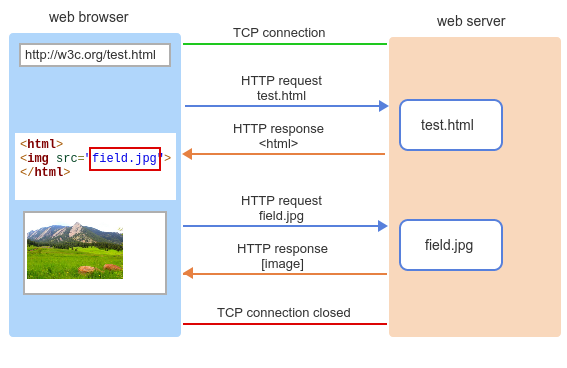
\includegraphics[width=\textwidth]{./imgs/httprequest.png}
        \end{figure}
    \end{minipage}
    \begin{minipage}{0.49\textwidth}
        \begin{itemize}
            \item \textbf{GET} \textrightarrow \
            \item \textbf{HEAD} \textrightarrow \
            \item \textbf{POST} \textrightarrow \
            \item \textbf{PUT} \textrightarrow \
            \item \textbf{DELETE} \textrightarrow \
        \end{itemize}
    \end{minipage}
\end{frame}

%
% Slide 2
%
\begin{frame}[fragile]
    \frametitle{Reading data from the internet}
    \begin{lstlisting}[language=Python, autogobble]
    import requests

    response = requests.get("https://www.google.com")
    \end{lstlisting} 
    \vfill
    \begin{enumerate}[A]
        \item From a Python program
        \item requests module: Given a URL, returns the document at that URL
    \end{enumerate}
    \pause
    Lets try this on PrairieLearn :D 
\end{frame}

\end{document}
